\documentclass{article}
\usepackage[utf8]{inputenc}
\usepackage[margin=2.6cm]{geometry}
\usepackage{float}
\usepackage{rotating}
\usepackage{caption}
\usepackage{subcaption}
\usepackage[round]{natbib}
\usepackage{setspace}
\onehalfspacing
\usepackage{tikz}
\usetikzlibrary{arrows,automata,positioning}

\title{
Resources availability, sociality, and the diversity of the female human life cycle.\\
PhD overall proposal}
\author{PhD candidate:\\
Pablo J. Varas Enríquez\\\\
Comittee:\\
Dr. Dieter Lukas\\
Dr. Monique Borgerhoff Mulder\\
Dr. Heidi Colleran}
\date{\today}

\begin{document}

\maketitle

\tableofcontents

\begin{abstract}
    The female human life cycle has evolved to have a long lifespan with a short reproductive period in between long juvenile and post-reproductive stages. Within these boundaries, humans can present diverse life cycles that can go from long lifespans and low reproductive output (e.g. post-demographic transition Japan) to short lifespans and high number of offspring (e.g. pygmies populations). These differences in the life cycle have been usually associated with the amount of resources that an individual has or the presence of some individuals in their social network, but how the link of both of them change the life cycle of an individual remains unclear. Here I expect to show how the interplay of the amount of resources and sociality may be key to understand why the female human life cycle varies. First, this project wants to understand how different combinations of resources and sociality change the life cycle of an individual. Afterwards, see how variations of these combinations through time diversify the female human life cycle. Finally, if the relationship between resources, sociality, and variations of the female human life cycle might change with the interplay of different types of resources (i.e. material, embodied, and relational). For this, dynamic stochastic programming models will be used to analyse how the sociality surrounding resources varies the female human life cycle. The results should demonstrate that sociality plays a buffering role in the effect of variations of resources in the female human life cycle. Furthermore, the resource-sociality dynamics during early stages of the life cycle would influence the current and future stages of the life cycle. Finally, material resource-related mechanisms would play the main role across the life cycle, while oscillations of them are buffered by embodied - while juvenile - and relational - once adult - resource-related mechanisms. In conclusion, the interplay and timing of resources and sociality explain the diversity of the female human life cycle. This dynamic would also prioritise material resources, which in turn would be buffered by relational and embodied resources.
\end{abstract}

\section{Introduction}

There are many developmental paths an individual can follow through its life cycle (i.e. life-history strategy), which is the basis of the diversity seen across the tree of life. The diversity of reproductive schedules can go from a couple to thousands offspring (e.g. eastern hemlock vs rain moth \citep{tindale1932revision,van2017lifetime} and mortality ones from lifespans of days to thousands of years (e.g. hairyback vs patagonian cypress \citep{balsamo1988life,lara19933620}). The different life-history strategies have usually been related to the limited resources an individual posses in its environment and how it allocates them \citep{stearns2000life}. Humans pose an interesting case regarding its life cycle due to the short reproductive period in comparison to their long lifespan, framed within long juvenile and post-reproductive stages \citep{kaplan2000theory}. Within these boundaries, humans present a high diversity of life-history strategies with populations where life spans are long and their reproductive output is low (e.g. post-demographic transition Japan \citep{de2017maximum}) while others have short lifespans and high reproductive output (e.g. pygmies populations \citep{migliano2007life}). The diversity in female human life-history strategies has also been associated with resource availability, specially in terms of longevity \citep{kaplan2003embodied}; while for fertility the relationship is more complex \citep{mulder1998demographic,sear2016understanding}. Additionally, sociality has been proposed as a way to understand the different life-history strategies among female human populations. Here, the presence or different members of a population in the social network of an individual have been associated with different female life-history strategies \citep{sear2011much}. Examples can be found in literature related to cooperative breeding, sibling competition, female conflict, among others \citep{ivey2000cooperative,nitsch2013elder,mace2012female}.However, both frameworks have not been able to explain what drives the diversity of female human life-history strategies. The interplay between the resources an individual possess and its sociality may be key to understand how the female human life cycle has evolved and diversified. Hence,  this project aims first to understand how different combinations of resources and sociality vary the life cycle of an individual. Afterwards, see how variations of these combinations through time might shape differently the female human life cycle. Finally, if the relationship between resources, sociality, and the diversity of the female human life cycle might change with the interplay of different types of resources.
\\\\
The average female human life cycle can be described as having a long lifespan, where a short reproductive period is squeezed between long juvenile and post-reproductive stages (see \ref{fig:1} for a graphical representation). Humans also show a higher fertility in comparison to other primates, despite the short reproductive period, due to its capacity of producing offspring within short interbirth intervals \citep{kaplan2000theory}. However, female humans can show diverse life-history strategies within these boundaries. They can show long life-expectancy (e.g. contemporary Japan $=$ 125 years old \citep{de2017maximum}, or short ones (e.g. pigmy populations $=$15-24 years old \citep{migliano2007life}). The number of offspring can also vary from childless or one offspring (e.g. contemporary East Asian countries \citep{jones2019ultra}) to fertility rates up to 11 children per woman (e.g. Hutterites \citep{eaton1953social}). The length of the juvenile period can also vary, where sexual maturity can be reached at 12 years old, as in Pumé population \citep{kramer2008early}, or at 16 years old, as in Senegal population \citep{simondon1997nutritional}. This variation can also be seen with age at first reproduction, where female humans can have their first offspring early in life (e.g. 15 years old in Pumé population \citep{kramer2008early}) or postpone their reproduction until they are as near to menopause as possible (e.g. women over 50 years old that use assisted reproductive technology \citep{salihu2003childbearing}). Female humans can also vary their interbirth intervals from short intervals (e.g. 2.75 years in Southern Ethiopia \citep{yohannes2011duration}) to longer ones in order to ensure their optimal reproductive success (e.g. 4 years in !Kung population \citep{jones1986bushman}). Finally, the age at last reproduction is one of the traits that most vary in female humans, where individuals from the Herero finish have their last offspring at 29 years old while those from the Ache population have it at 42 years old \citep{towner2016women}. Therefore, the female human life cycle can be highly flexible within the boundaries of long juvenile and post-reproductive periods, with a short reproductive stage, allowing indivduals to adapt their life-history strategies to different scenarios.
\\\\
\begin{figure}[H]
    \centering
    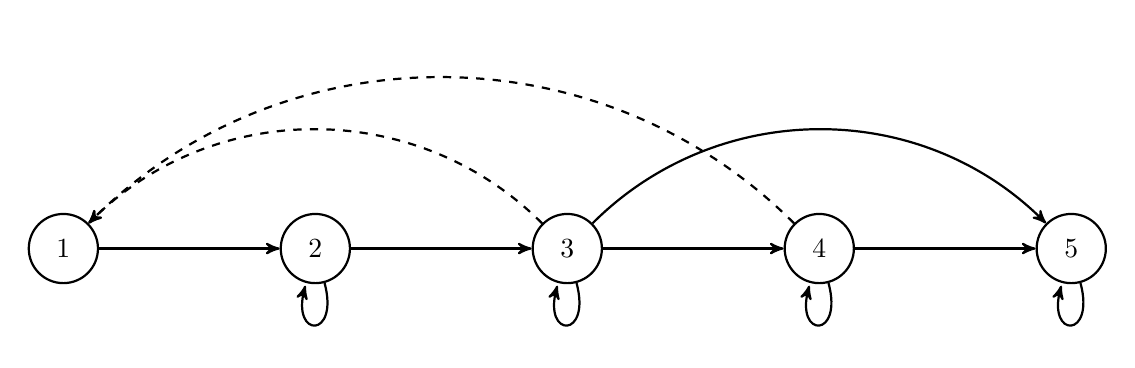
\begin{tikzpicture}[->,>=stealth',auto,node distance=3.2cm,
thick]
\tikzstyle{every state}=[fill=white,shape=circle,draw,thick,text=black, text centered, text width=0.5cm, align=center]

\node[state]		(A)              {1};
\node[state]        (B) [right of=A] {2};
\node[state]        (C) [right of=B] {3};
\node[state]        (D) [right of=C] {4};
\node[state]		(E) [right of=D] {5};

\path (A) 	edge			(B)
(B)	edge			(C)
(C)	edge			(D)
(D)	edge			(E)
(C) edge[bend right=-45] (E)
(C) edge[dashed,bend left=-45] (A)
(D) edge[dashed,bend left=-45] (A)
(B) edge[loop below] (B)
(C) edge[loop below] (C)
(D) edge[loop below] (D)
(E) edge[loop below] (E);
\end{tikzpicture}
\caption{Life cycle graph of the human life cycle in five stages. 1 is the newborn stage, 2 the sexually immature stage (i.e. juvenile), 3 the reproductive non-breeding stage (i.e. adulthood), 4 the reproductive breeding stage (i.e. parenthood), and 5 the post-reproductive stage (i.e. elderhood). The thick arrows refers to the transition from one stage to the other or staying in the same one for a period of time, while the dashed one refers to offspring production. A newborn is produced either when an individual transition from stage 3 to 4 or when an individual remains in stage 4 (dashed arrow).}
    \label{fig:1}
\end{figure}

Life history theory is the main framework used to understand the life cycle of an organism and its diversity across the tree of life,  from an evolutionary perspective. Life history theory aims to explain the differences in the survival, reproduction, growth, and development of organisms based on a differentiated individual allocation of resources depending on environmental conditions \citep{stearns2000life}. Humans are no exception, and several studies in evolutionary anthropology have used this framework to understand the different life-history strategies that female humans show \citep{mace2000evolutionary,borgerhoff2012human}. The main life-history trade-offs that have been addressed in human populations are quantity vs quality of offspring, reproduction now vs later, and reproductive vs (extra) somatic investment \citep{hill1999life}. Quantity vs quality offspring trade-off refers to the trade-off an individual faces on either investing resources to have a large number of “low-quality” offspring or a few “high-quality” ones. The trade-off reproduce now vs later refers to the moment an individual faces to either postpone reproduction or not, mainly related to its probability to survive later in life. The trade-off between reproduction and (extra) somatic investment alludes to the allocation of resources an individual does towards its offspring or to its own survival and development. Among these trade-offs, the quantity versus quality offspring trade-off has received major attention by itself, leaving few space to analyse the possibility of an interplay of different life-history trade-offs and/or the role of other trade-offs as well \citep{lawson2016offspring}. Furthermore, this situation has led to address mainly the relationship between the amount of resources available and offspring production. This approach usually does not question how and when resources are available but focuses more on how much there are.
\\\\
Competition and cooperation have been used to address how sociality may influence the life history trade-offs an individual faces across its life cycle \citep{cant2008reproductive,kramer2005children}. On the one hand, studies on competitive dynamics have focused on reproductive conflict, where intrasexual competition is high between generations \citep{mace2012female,lahdenpera2012severe} and co-residency patterns \citep{pettay2016costly}. Also, sibling competition has been studied in humans, by addressing how the competition among the offspring of an individual influences resource allocation and parent fitness \citep{lawson2009trade}. An example can be seen in rural Ethiopia where land inheritance may increase competition, decreasing productivity and reproductive success of younger siblings \citep{gibson2011land}. On the other hand, the relationship of cooperation and the female human life-history strategy has been framed within the cooperative breeding model, where individuals other than parents help rearing their offspring \citep{hrdy2007evolutionary}. Evidence has been found in rural Ireland, where siblings would suppress their reproduction to take care of the land for the older sibling that is inheriting the land \citep{strassmann1998ecological} while in Mayan and Pumé population infant care is shared between the mother (57\%) and other relatives (43\%) \citep{kramer2018infant}. Most likely, elements of competition and cooperation coexist in human populations, depending on such factors as resource availability \citep{mulder2007hamilton} or genetic relatedness \citep{strassmann2011cooperation}. 
\\\\
Despite the large amount of research done within the competition/cooperation dichotomy, there is no consensus regarding the influence of competitive and cooperative dynamics in the female human life cycle, due to methodological and theoretical issues. Methodologically, there is a high variety of outcome variables used in these studies that are not standardized and makes it difficult to compare results between studies and populations (e.g. compare   individual survival with number of surviving offspring or child anthropometrics) \citep{brown2002reconsidering}. Additionally, many studies use kin presence to address competitive or cooperative dynamics depending on the direction of the relationship between the kin member and the life-history trait of interest (negative = competition and positive = cooperation) \citep{sear2011much}, leaving in a black box the mechanisms that could explain these relationships. Theoretically, the lack of consensus has lead to the development of multiple models trying to explain the female human life cycle, such as the embodied capital model - or its more specific formulation, the pooled energy budget model - to explain the long juvenile period \citep{kaplan2000theory,kramer2010pooled}; the cooperative breeding model to explain the large number of offspring and short interbirth intervals \citep{kramer2005children}; or the grandmother hypothesis to explain the post-reproductive lifespan \citep{hawkes2013grandmothers}. This scenario has led to multiple hypotheses of the relationship between competition/cooperation and the female human life cycle, focusing only on specific stages of the life cycle. Related to this last point, many of these models and research do not consider the influence of social interactions in early stages of the life cycle, leaving out of the equation the possibility that what can be seen in one stage can be reversed or compensated at a later stage \citep{mulder1998demographic}. Therefore, there is a need for unifying life-history, demographic, and sexual selection models to understand the black box in which the link between resource availability and sociality might vary the life-history strategy of a female human, behind the curtains of cooperation and competition.
\\\\
Resource transfers, understood as the social interactions where an individual gives or receives a resource, might be a starting point to understand how sociality and resources shape the life-history strategies of female humans. In other species, resource transfers, such as food provisioning and alloparenting in meerkats \citep{clutton2016meerkats}, territorial defense and predator detection in acorn woodpecker \citep{koenig2019does}, and bequeathal in kangaroo rats \citep{jones1986survivorship} have been associated with variations in the survival and reproductive dynamics of an individual life cycle. For humans, it has been suggested that resource transfers are crucial to understand the survival timing in the female human life cycle, with high early mortality and post-reproductive lifespan \citep{lee2003rethinking,lee2008sociality,chu2006co}. Resource transfers might also be crucial in the reproductive timing of humans, where they not only relate to offspring survival until sexual maturity via alloparenting, but also to transfers that might enhance the mating success of the offspring (e.g. bridewealth) \citep{jones2015resource}. Hence, disentangling how resource transfers shape an individual life cycle could help to understand the role of social interactions in the variations of human survival, reproductive, and developmental timing.
\\\\
The mechanisms by which the amount of resources a female human possess links to its life cycle have been related to production and consumption. The ability of producing more than what is consumed during adulthood has been the main feature by which researchers have explained the long juvenile and post-reproductive periods in the female human life cycle \citep{kaplan2000theory}. Kaplan and collaborators also suggest that the high amount of resource production also allows female humans to have short interbirth intervals, leading to a high reproductive output in short reproductive lifespans when compared to other primates. Additionally, the surplus of resource production combined with resource transfers can lead to the accumulation of resources through several generations (e.g. land, body weight, social status) \citep{mulder2009intergenerational}. These kinds of mechanisms have led to propose that the resource accumulation of a human in one life cycle can influence fitness benefits for itself, its offspring, grand-offspring, and beyond \citep{rogers1990evolutionary,boone1999more,goodman2012low}. Thus, the interplay of resource transfers with production, consumption, and accumulation might be a good starting point to understand how resources and sociality may influence the life-history strategy of an individual, specially at different points of its life cycle.
\\\\
However, the relationship of resources and sociality with the female human life cycle might also vary depending on the type of resources. Research on female human life-history strategies and the interplay between sociality and resource availability have mainly focused on material resources due to evidence that economic conditions may mediate reproductive behaviour \citep{shenk2013model}. However, there is also evidence that embodied resources also played a role, such as the influence of parental educational level, and their investment in the education of their offspring, in variations on the reproductive behaviour of the descendants \citep{kaplan1996theory,snopkowski2014synthetic,snopkowski2016pathways}. Furthermore, relational resources seem to also play a role in the female human life-history strategies, where social status and prestige across generations may be crucial to understand reproductive and survival schedules \citep{boone1999more,shenk2016status}. Examples can be seen in Agta and BaYaka hunter-gatherers, where women with high relational resources also present high fertility \citep{chaudhary2016competition,page2017hunter}. The ways in which the interplay of these types of resources and how they relate to the life-history strategies of female humans remain unclear. One of the few examples can be seen in Mpimbew population, where material and relational resources may be more important than embodied resources to ensure child survival \citep{mulder2011understanding}. Hence, the relationship between resources and sociality might need to account for different types of resources to explain the variations of life-history strategis in female human populations.
\\\\
In conclusion, this project aims to understand how and when the sociality and the resources that a female individual possess might shape its life-history strategy, and how this vary with different types of resources at different stages of life. Hence, the research questions of this project are \textbf{A) how does the interplay of resources and sociality shape the life-history strategy of a female human individual?} The life-history strategy of a female individual would vary mainly due to changes in the amount of resources that she possess, while sociality would play a buffering effect. An individual would increase its longevity and decrease its reproductive output as the amount of resources increase. However, sociality would buffer the resources effect since it would be spread the amount of resources in the population via transfers dynamics (\ref{fig:2}). \textbf{B) How does variations of the relationship between resources and sociality across the life cycle influence the life-history strategy of a female individual?} The female human life-history strategy would vary depending on the variability of resources and sociality during the early stages of the life cycle. Individuals would show a life-history more similar to the one experienced in their early stages of the life cycle if they would have more stable amount of resources and sociality during those stages. Sociality would have a buffering effect on oscillations of the amount of resources across the life cycle. Finally, \textbf{C) how the relationship of resources and sociality with the female human life-history strategies changes depending on the interplay of material, embodied, and relational resources?} Material resources would have the main influence in the relationship between resources, sociality, and the female human life-history strategy. Embodied resources would play a buffering effect under oscillations of material resources during the early stages of the life cycle, and relational one in the later ones.

\begin{figure}[H]
     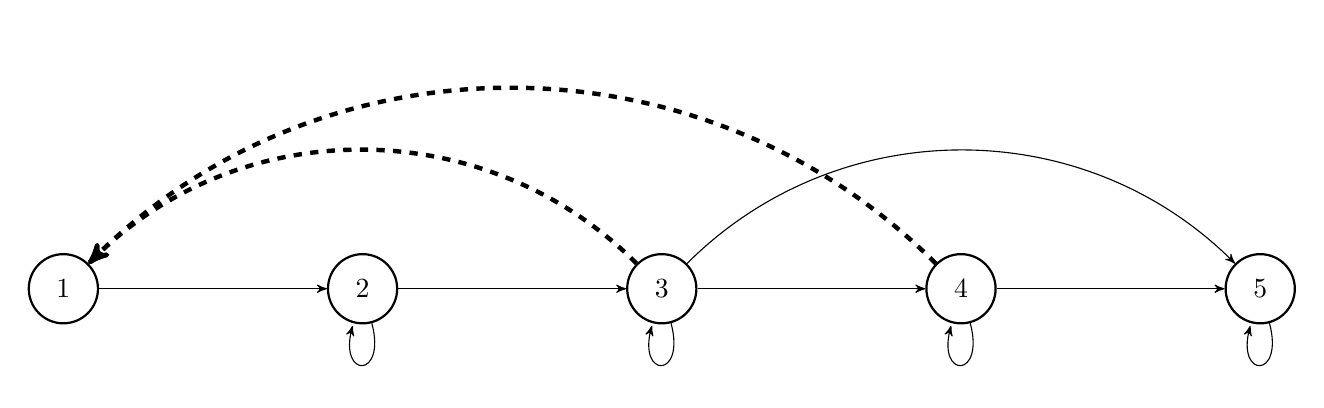
\begin{tikzpicture}[->,>=stealth',auto,node distance=3.8cm,
thin]
\tikzstyle{every state}=[fill=white,shape=circle,draw,thick,text=black, text centered, text width=0.5cm, align=center]

\node[state]		(A)              {1};
\node[state]        (B) [right of=A] {2};
\node[state]        (C) [right of=B] {3};
\node[state]        (D) [right of=C] {4};
\node[state]		(E) [right of=D] {5};

\path 
(A) edge			(B)
(B)	edge			(C)
(C)	edge			(D)
(D)	edge			(E)
(C) edge[bend right=-45] (E)
(C) edge[dashed,ultra thick,bend left=-45] (A)
(D) edge[dashed,ultra thick,bend left=-45] (A)
(B) edge[loop below] (B)
(C) edge[loop below] (C)
(D) edge[loop below] (D)
(E) edge[loop below] (E);
\end{tikzpicture}
\hfill
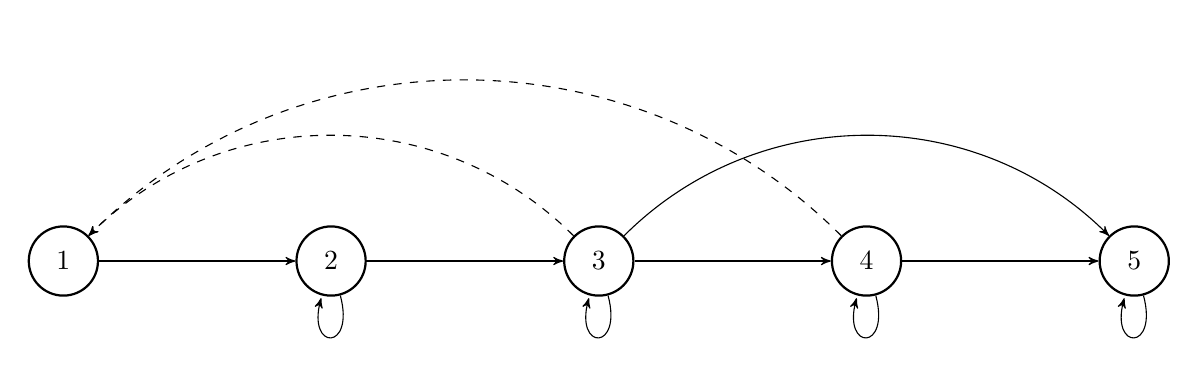
\begin{tikzpicture}[->,>=stealth',auto,node distance=3.4cm,
thin]
\tikzstyle{every state}=[fill=white,shape=circle,draw,thick,text=black, text centered, text width=0.5cm, align=center]

\node[state]		(A)              {1};
\node[state]        (B) [right of=A] {2};
\node[state]        (C) [right of=B] {3};
\node[state]        (D) [right of=C] {4};
\node[state]		(E) [right of=D] {5};

\path (A) 	edge			(B)
(B)	edge			(C)
(C)	edge			(D)
(D)	edge			(E)
(C) edge[bend right=-45] (E)
(C) edge[dashed,bend left=-45] (A)
(D) edge[dashed,bend left=-45] (A)
(B) edge[loop below] (B)
(C) edge[loop below] (C)
(D) edge[loop below] (D)
(E) edge[loop below] (E);
\end{tikzpicture}
\hfill
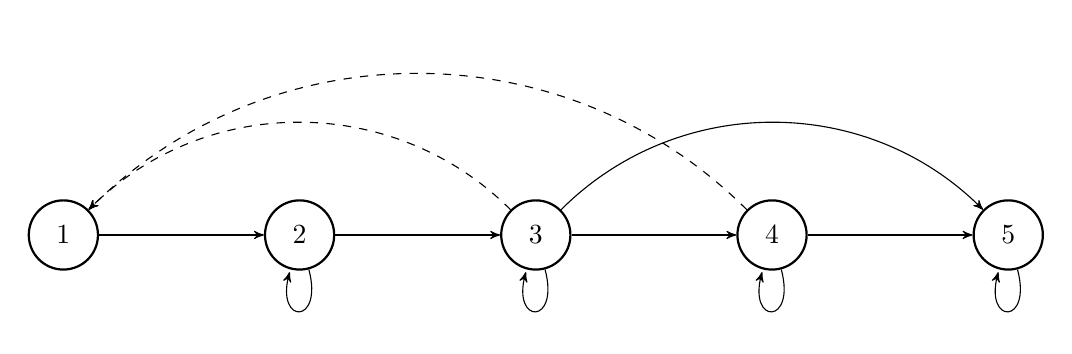
\begin{tikzpicture}[->,>=stealth',auto,node distance=3cm,
thin]
\tikzstyle{every state}=[fill=white,shape=circle,draw,thick,text=black, text centered, text width=0.5cm, align=center]

\node[state]		(A)              {1};
\node[state]        (B) [right of=A] {2};
\node[state]        (C) [right of=B] {3};
\node[state]        (D) [right of=C] {4};
\node[state]		(E) [right of=D] {5};

\path (A) 	edge			(B)
(B)	edge			(C)
(C)	edge			(D)
(D)	edge			(E)
(C) edge[bend right=-45] (E)
(C) edge[dashed,bend left=-45] (A)
(D) edge[dashed,bend left=-45] (A)
(B) edge[loop below] (B)
(C) edge[loop below] (C)
(D) edge[loop below] (D)
(E) edge[loop below] (E);
\end{tikzpicture}
\hfill
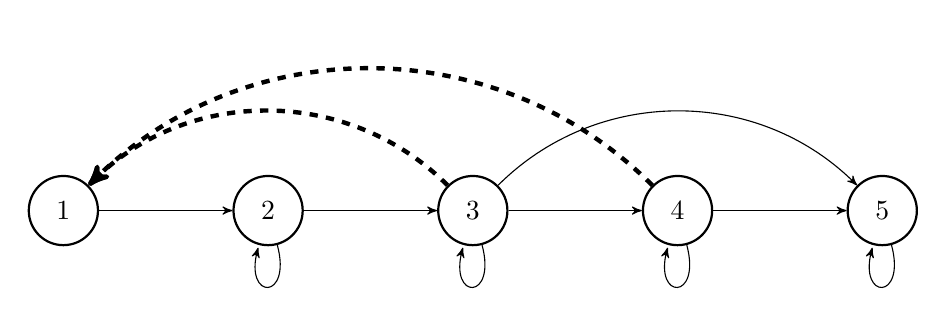
\begin{tikzpicture}[->,>=stealth',auto,node distance=2.6cm,
thin]
\tikzstyle{every state}=[fill=white,shape=circle,draw,thick,text=black, text centered, text width=0.5cm, align=center]

\node[state]		(A)              {1};
\node[state]        (B) [right of=A] {2};
\node[state]        (C) [right of=B] {3};
\node[state]        (D) [right of=C] {4};
\node[state]		(E) [right of=D] {5};

\path (A) 	edge			(B)
(B)	edge			(C)
(C)	edge			(D)
(D)	edge			(E)
(C) edge[bend right=-45] (E)
(C) edge[dashed,ultra thick,bend left=-45] (A)
(D) edge[dashed,ultra thick,bend left=-45] (A)
(B) edge[loop below] (B)
(C) edge[loop below] (C)
(D) edge[loop below] (D)
(E) edge[loop below] (E);
\end{tikzpicture}
\caption{Life cycle graphs of the human life cycle under different combinations of resources and sociality. 1 is the newborn stage, 2 the sexually immature stage (i.e. juvenile), 3 the reproductive non-breeding stage (i.e. adulthood), 4 the reproductive breeding stage (i.e. parenthood), and 5 the post-reproductive stage (i.e. elderhood). The thick arrows refers to the transition from one stage to the other or staying in the same one for a period of time, while the dashed one refers to offspring production. A newborn is produced either when an individual transition from stage 3 to 4 or when an individual remains in stage 4. The length of the transition arrows refer to different lengths of lifespan while the thickness of dashed arrows refers to the number of offspring produced in that life cycle. The first life cycle is the one for high amount of resources and sociality, the second one to high amount of resources but low sociality, the third one to low resources but high sociality, and the fourth one to low resources and sociality.}
    \label{fig:2}
\end{figure}


\section{Methodology}

Research related to the influence of the interplay of sociality and resources with female life-history strategies have combined life-history theory and economic models. This approach is based in a consensus that human reproductive behaviour might be primarily driven by rational economic decisions \citep{jones2015resource}. On the one hand, the embodied capital theory suggests that the surplus of resource production during adulthood allows the evolution of the female human life cycle \citep{kaplan2000theory}. This model proposes that the difference between resource production and consumption allows high parental investment, translated in short interbirth intervals and long post-reproductive periods for the parents and long juvenile periods for their offspring. Furthermore, the pooled energy model deepens in this framework by suggesting that alloparenting from individuals of different generations would allow to decrease the load of parental investment \citep{kramer2010pooled}. On the other hand, resource transfer theory poses that intergenerational transfers would play a major role in the mortality and fertility schedules of human populations. \cite{lee2003rethinking} suggests that age-specific mortality is proportional to the remaining reproductive value and resource transfers made at later ages, predicting the early-life and later-life mortality patterns characteristics of the female human life cycle. Additionally, \cite{chu2006co} model shows that intergenerational transfers coevolve with low mortality, since adults are more efficient to produce energy, which is transfered to juveniles, who are more efficient to turn that energy into body size, allowing lower mortality. Hence, these models show that the human life cycle evolves from the interplay of resources and sociality. However, they do not explain the conditions under which the life cycle varies.
\\\\
Other limitations of these models rely on two main assumptions. First, all resources in a sharing group must be consumed, there is no possibility for accumulation or waste of resources \citep{lee2008sociality} unless it is for body size \citep{chu2006co,kaplan2003embodied}. Hence, they do not account for the influence of accumulated resources  in later stages of the life cycle or further generations \citep{goodman2012low}. Second, the sharing dynamics in these models (i.e. net transfers) are assumed to be the difference between production and consumption, where positive values imply giving resources while negative ones mean receiving them \citep{lee2003rethinking,lee2008sociality,chu2006co}. Therefore, the social interactions surrounding resources are a by-product of the capacity of resource production and consumption by an individual.
\\\\
Dynamic sochastic programming models might be a modelling approach able to tackle the issues pending from previous models. These models account for the current stage of an individual and its possible changes according to the actions and environment of an individual, allowing to analyse the optimal individual behaviour and the different trade-offs behind its variation considering the stage-specific constraints of the individual \citep{houston1988dynamic,clark2000dynamic}. Dynamic stochastic programming models have been used before to explain optimal life-history strategies in different human populations. \cite{anderies1996adaptive} used this approach to predict maximization of interbirth intervals among !Kung women by including mortality schedules, backload and foraging success. \cite{mace1996have} developed a model to understand the optimal family size among Gabbra, based on household wealth and the number of offspring an individual has. Also, \cite{luttbeg2000marry} applied this framework to understand if Kipsigis men decide to marry or not in order to maximize the number of offspring or the amount of wealth they can transfer to them, based on the value of livestock, number of wives and children, and amount of land. Finally, \cite{thomas2015dynamic} used these models to understand how interbirth intervals vary depending on sibling competition and mortality risks. Therefore, a dynamic stochastic programming model may allow to understand the variations on the life-history trajectory of an individual depending on the resources available, and the ways it is available, at different points in life.

\section{Expected product}

\begin{itemize}
    \item The interplay of resources and sociality explain the diversity of female human life-history strategies.
    \begin{itemize}
        \item This paper should focus on the development of an optimality model to show that there are different optimal life-history strategies depending on different ways in which resources and sociality interplay. Also, show the results from testing the model with empirical data.
    \end{itemize}
    \item Variations of resources and sociality through time change female human optimal life-history strategy.
    \begin{itemize}
        \item Here, the idea is to show the second model, which analyze how variations of resources and sociality in different stages of the life cycle change the optimal life-history strategy. Also, show the results from testing the model with empirical data.
    \end{itemize}
    \item Differences in the link between resources, sociality, and female human life-history strategies due to material, embodied, and relational resources.
    \begin{itemize}
        \item Here, the idea is to show how the relationship between resources, sociality, and the optimal life-history strategy might differ when considering different types of resources (i.e. material, embodied, relational). The publication would have, again, a model+data analysis structure.
    \end{itemize}
\end{itemize}

\section{Schedule}

\begin{sidewaystable}[ht!]
\centering
\captionof{table}{Year 1}
\begin{tabular}{ l*{12}{c}r } 
 \hline
 Phase & Oct '19 & Nov '19 & Dec '19 & Jan '20 & Feb '20 & Mar '20 & Apr '20 & May '20 & Jun '20 & Jul '20 & Aug '20 & Sep '20 & Oct '20 \\
 \hline
 Proposal & X & X & X & X & X & X & X & X & X & X & X & X & X \\
 \hline
\end{tabular}
\hspace{\parskip}
\captionof{table}{Year 2}
\begin{tabular}{ l*{12}{c}r  } 
 \hline
 Phase & Oct '20 & Nov '20 & Dec '20 & Jan '21 & Feb '21 & Mar '21 & Apr '21 & May '21 & Jun '21 & Jul '21 & Aug '21 & Sep '21 & Oct '21 \\
 \hline
 Model 1 dev. & X & X & X & X & & & & & & & & & \\
 Model 1 ansis. &  &  &  & X & X & X & X & & & & & & \\
 Paper 1 subm. &  & X &  & X & & X & X & X & & & & & \\
 Model 2 dev. & & & & & & & X & X & X & X & & & \\
 Model 2 ansis. &  & & & & & & & & X & X & X & X & \\
 Paper 2 subm. & & & & & & & & & X & & X & X & X \\
 Model 3 dev. & & & & & & & & & & & & X & X \\
 \hline
\end{tabular}
\hspace{\parskip}
\captionof{table}{Year 3}
\begin{tabular}{ l*{11}{c}r  } 
 \hline
 Phase & Oct '21 & Nov '21 & Dec '21 & Jan '22 & Feb '22 & Mar '22 & Apr '22 & May '22 & Jun '22 & Jul '22 & Aug '22 & Sep '22\\
 \hline
 Model 3 dev. & X & X & X & & & & & & & & & \\
 Model 3 ansis. &  & X & X & X & X & & & & & & & \\
 Paper 3 subm. &  & X &  & X & X & X & & & & & & \\
 Thesis subm. & & & & & & & X & X & X & X & & \\
 Thesis def. &  & & & & & & & & & X & X & X \\
 \hline
\end{tabular}
\end{sidewaystable}

\clearpage

\bibliographystyle{apalike}
\bibliography{proposal_ref}

\end{document}
